\subsection{Theoretical Background}

There is not a lot of complex theory behind simple C++ style template expansion, in theory all you
have to do is create a new class or method where you have replaced every instance of a template
parameter with the type value of the parameter.  If you for example have a template class
\textbf{Foo$\langle$T,V$\rangle$} and you invoke it by calling \textbf{bar = new
Foo$\langle$Int,Bool$\rangle$}, all you have to do is copy the class definition for
\textbf{Foo$\langle$T,V$\rangle$} and replace all T:s with Int and V:s with Bool. For simple
programs this can be done by hand without much effort, but for more complex programs it can be hard
to calculate which ``real'' versions of the template classes are necessary, and expanding them all
might be impossible. We've solved this problem by iteratively searching for template references and
expanding the class or method templates one by one. In the end the result is a normal KOOL source
file without any of our extended grammar.

\subsection{Implementation Details}

We make use of some properties of the KOOL language and our template specification to make the
implementation simple:

\begin{itemize}
    \item All classes are declared at the top level
    \item All methods are declared at the top level of a class
    \item The language has no inclusion or import feature
    \item Template parameters may not shadow class declarations
    \item Method template parameters may not shadow class template parameters
\end{itemize}

These properties allow for easy lookup of templates, since for example there is no need to search
for template declarations in statements. This makes the implementation easy --- in fact, class
templates can be completely expanded as a separate phase before name analysis since the name lookup
in this case is so simple. Method template expansion is done as part of the type checking phase,
since we need to know the receiver type of a method call before we can look up the method template.
The last two points mean we can replace template parameters in expanded templates based on name
alone, without needing to resolve whether a type name refers to a concrete class or a type
parameter.

Since templates may reference themselves or other templates, template expansion is done iteratively.
The class template expansion phase loops back to itself if any templates were expanded, and the
method template expansion subphase loops back to class template expansion if any templates were
expanded. \figref{compiler-flowchart} illustrates the flow between compiler phases.

\begin{figure}[hbtp]
  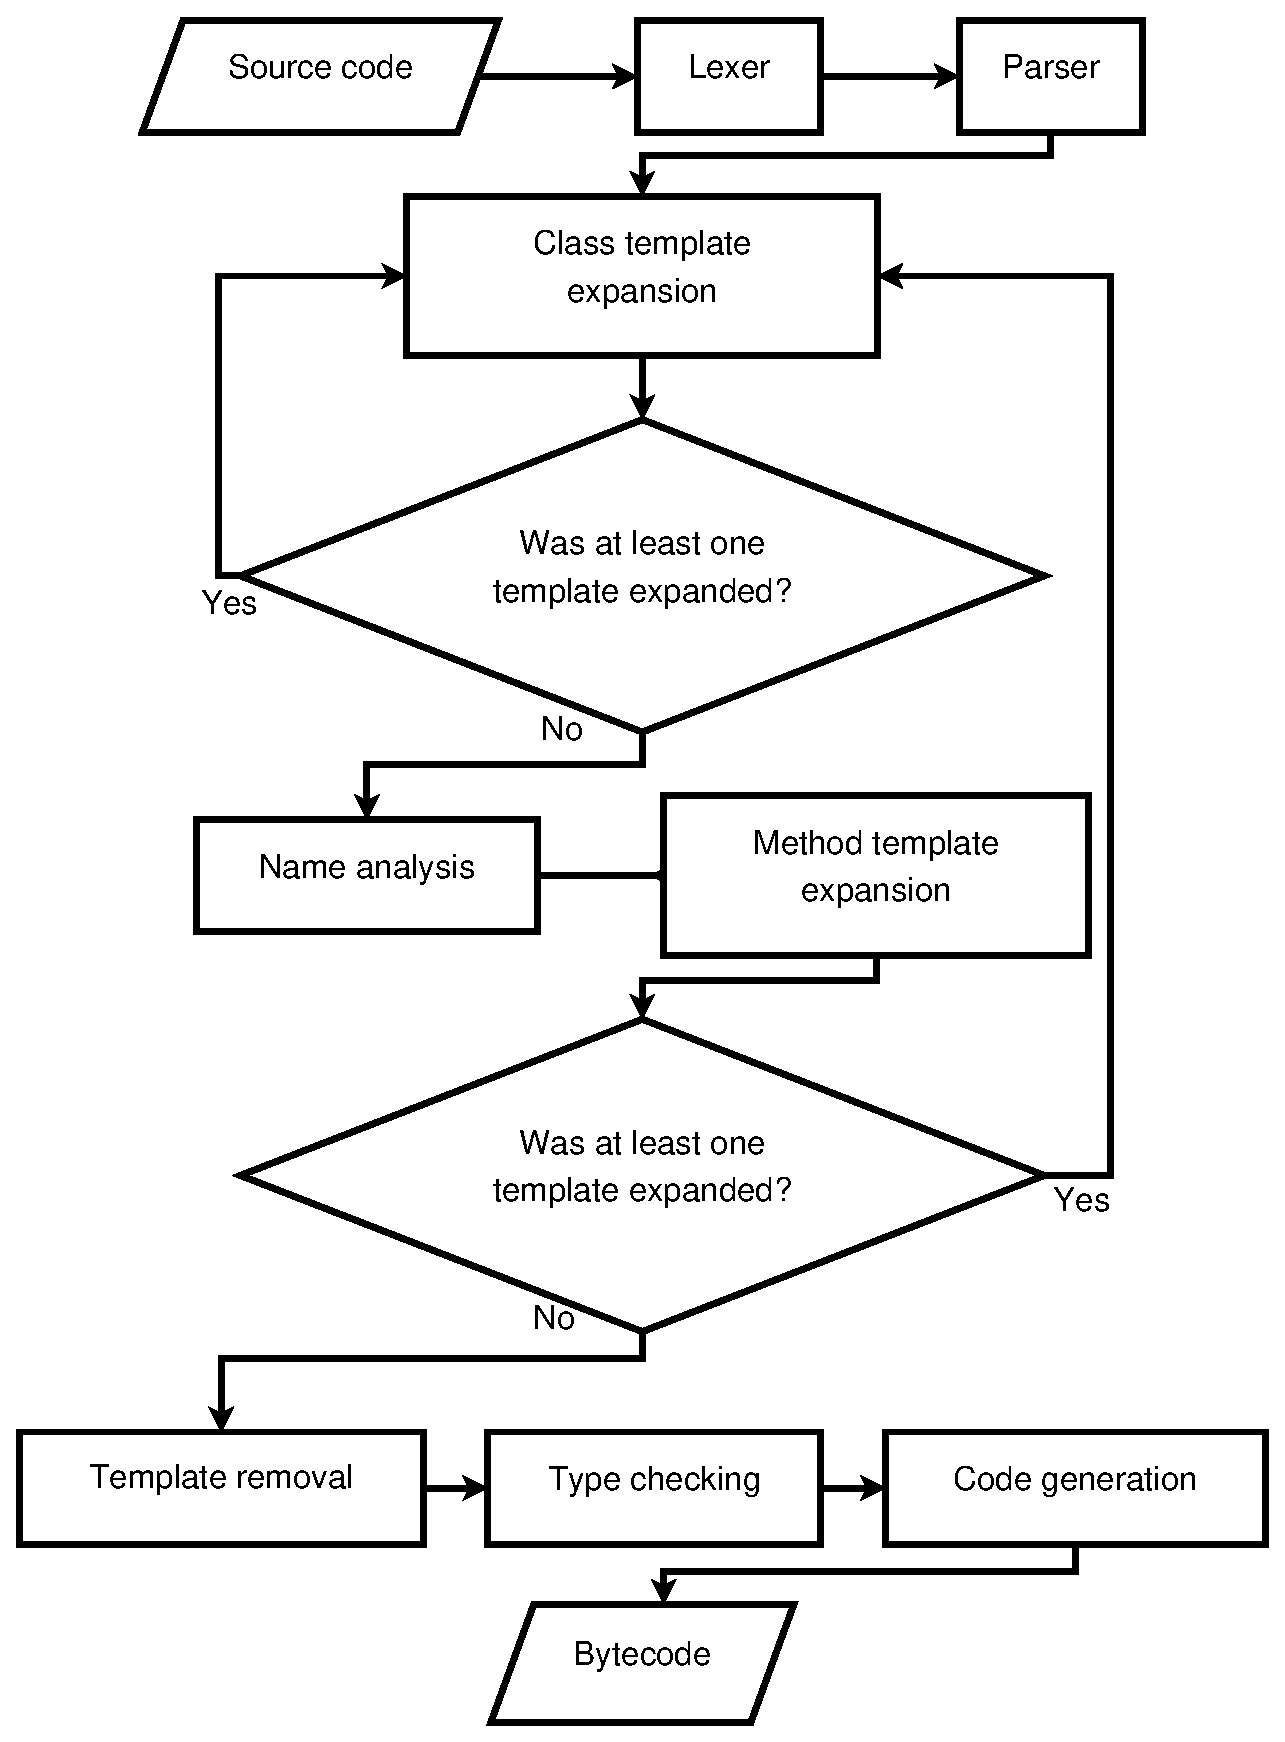
\includegraphics[width=0.5\textwidth]{compiler-flowchart}
  \caption{Compiler phases flow diagram. Since templates may reference other templates that may in
    turn need expansion, the template expansion phases must be iterated until all template
    references have been replaced with references to concrete expanded types or methods.}
  \label{fig:compiler-flowchart}
\end{figure}

In each iteration of the template expansion phases, only the leaves in each tree of template
arguments is expanded. This helps ensure that the types passed as template arguments are always
complete --- for instance, consider the template reference
\textbf{Maybe\tmpl{LinkedList\tmpl{Int}}}. If we were to expand the \textbf{Maybe} template first,
we would need to account for the fact that its type argument is also a template type. By instead
only expanding the innermost template references --- \textbf{LinkedList\tmpl{Int}} in this case ---
in each iteration, the procedure is made simpler because we know the type arguments will always be
concrete types.


\emph{Describe all non-obvious tricks you used. Tell us what you thought was hard and
why. If it took you time to figure out the solution to a problem, it probably
means it wasn't easy and you should definitely describe the solution in details
here. If you used what you think is a cool algorithm for some problem, tell us.
Do not however spend time describing trivial things (we know what a tree traversal
is, for instance).}

\emph{After reading this section, we should be convinced that you knew what you were
doing when you wrote your extension, and that you put some extra consideration
for the harder parts.}
